\section{Model Serving}

Dalam makalah ini akan dibahas secara lebih mendalam terkait Model Serving.
Hal-hal yang akan dibahas meliputi bagaimana metode-metode yang ada dalam melakukan serving dan teknologi apa yang digunakan untuk melakukan \textit{deployment} model tersebut.

Berdasarkan~\cite{mlopsorg}, lima jenis \textit{serving pattern} yang biasa digunakan untuk membuat layanan dari model:
\begin{enumerate}
  \item Model-as-Service
  \item Model-as-Dependency
  \item Precompute Serving
  \item Model-on-Demand
  \item Hybrid Serving
\end{enumerate}

\subsection{Model-as-Service}

\begin{figure}
  \centering
  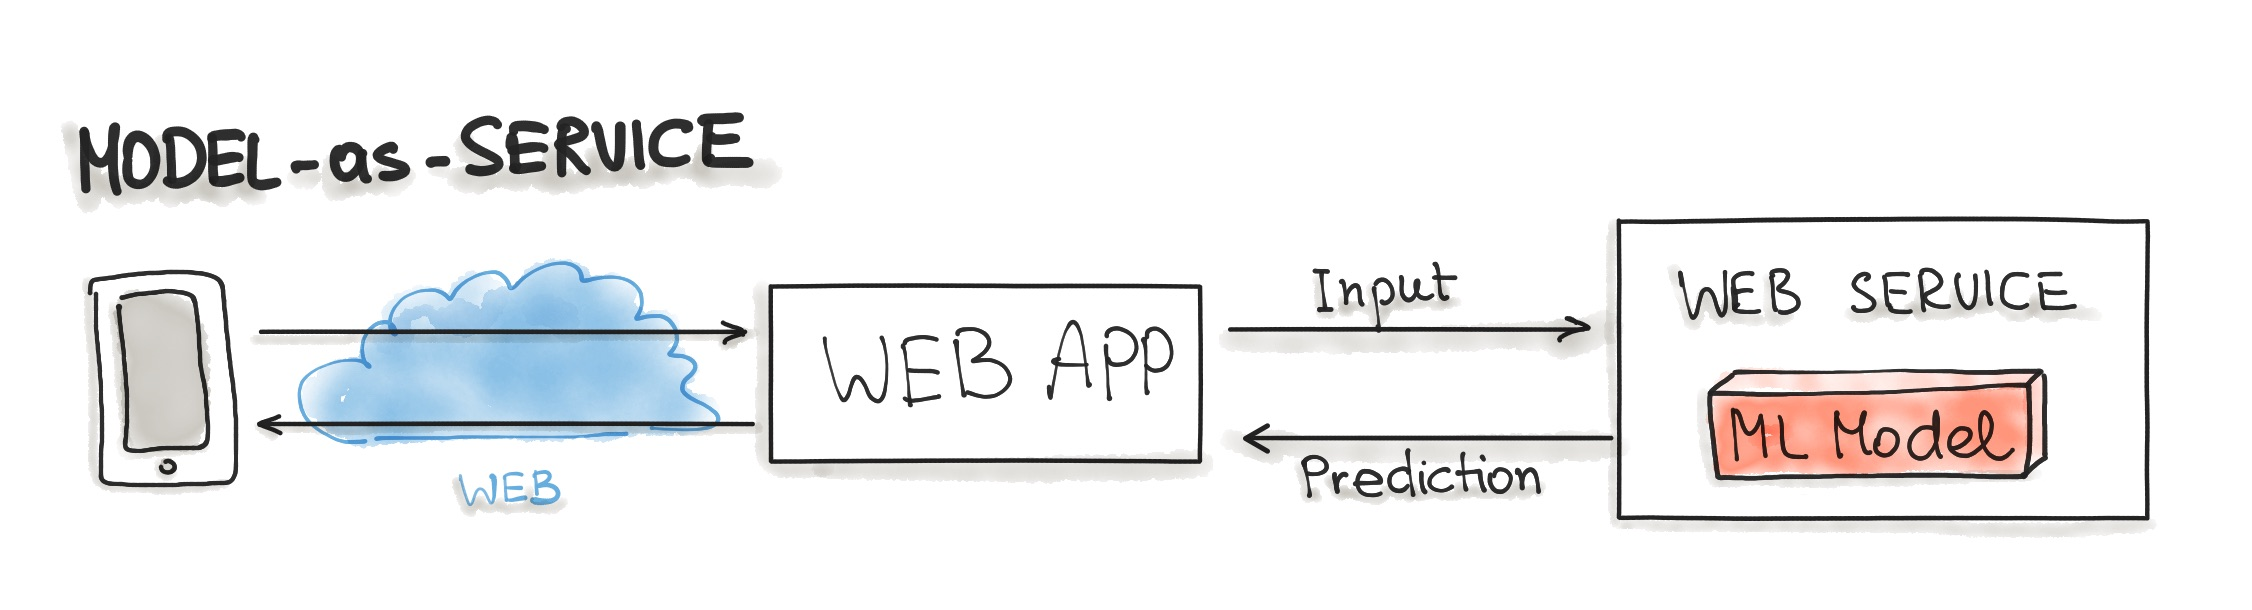
\includegraphics[width=0.8\textwidth]{02-model-as-service.jpg}
  \caption{Ilustrasi Model-as-Service (Sumber:~\cite{book-handsonml})}
\end{figure}

Serving pattern ini adalah metode yang paling sederhana.
Pada dasarnya, model yang sudah ada akan dibungkus dengan sebuah interface agar dapat dilakukan RPC terhadap model tersebut.
Teknologi yang umum digunakan biasanya seperti REST API dan gRPC, namun metode-metode RPC lainnya bisa juga digunakan.

\subsection{Model-as-Dependency}

\begin{figure}
  \centering
  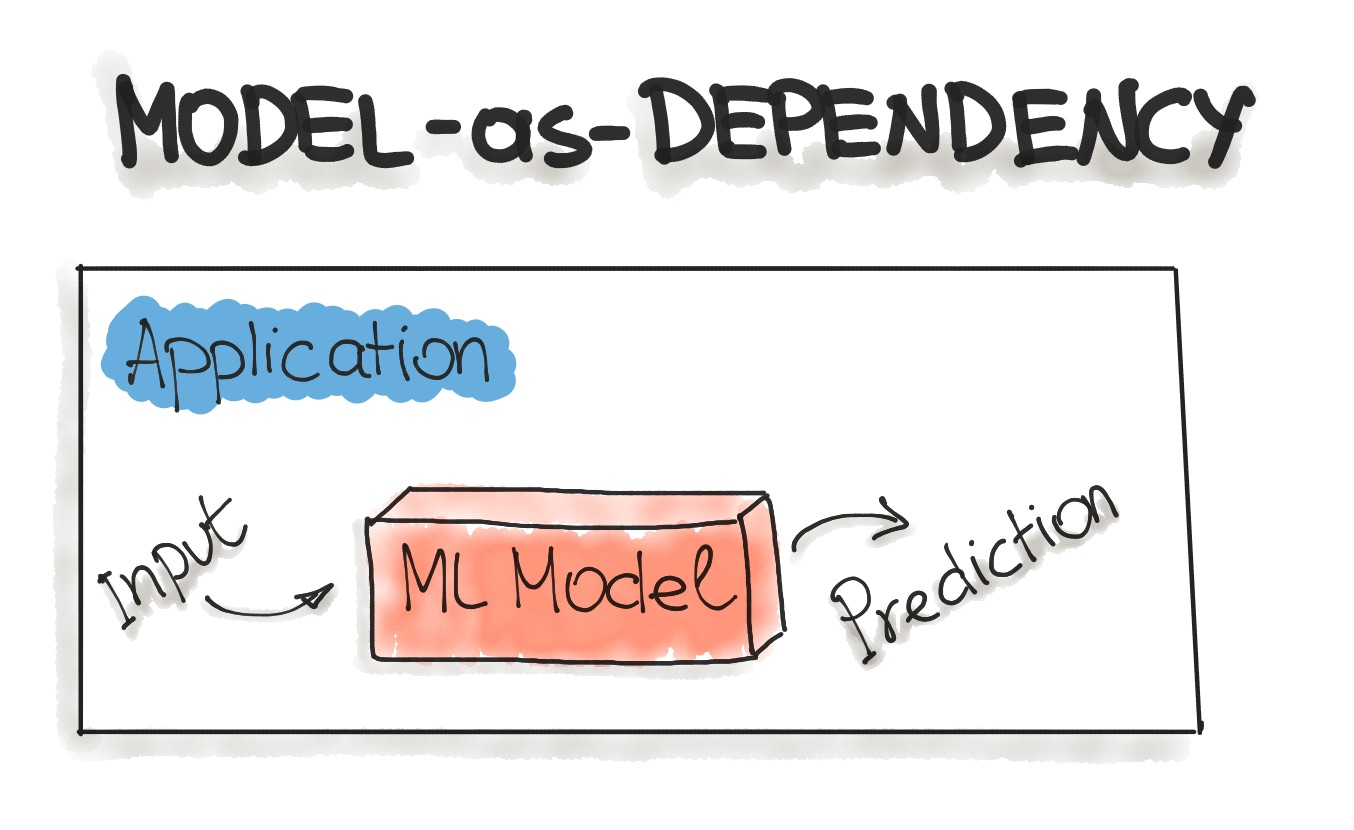
\includegraphics[width=0.8\textwidth]{02-model-as-dependency.jpg}
  \caption{Ilustrasi Model-as-Dependency (Sumber:~\cite{book-handsonml})}
\end{figure}

Serving pattern serupa dengan Model-as-Service, tetapi perbedaan utamanya adalah di mana model tersebut menjadi dependency dari layanan yang dibuat secara internal, bukan melakukan \textit{deployment} secara terpisah untuk model tersebut.
Pattern ini akan digunakan apabila model akan digunakan sebagai satu bagian dari layanan yang lebih besar.

\subsection{Precompute Serving}

\begin{figure}
  \centering
  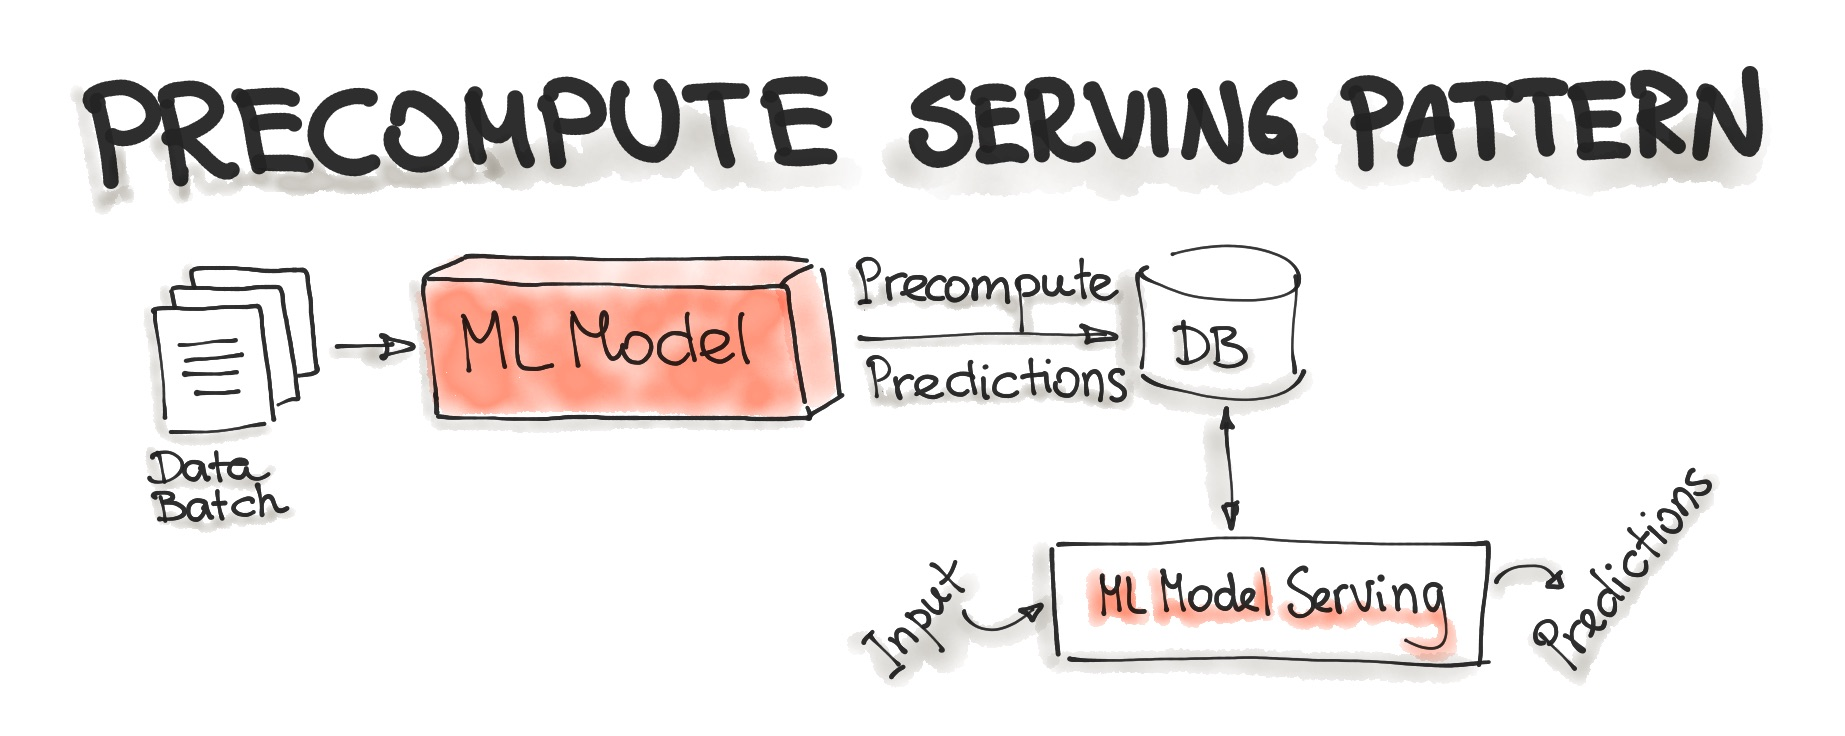
\includegraphics[width=0.8\textwidth]{02-precompute-serving-pattern.jpg}
  \caption{Ilustrasi Precompute Serving Pattern (Sumber:~\cite{book-handsonml})}
\end{figure}

Sesuai namanya, model akan digunakan untuk melakukan prekomputasi menggunakan model.
Hasil dari prekomputasi yang dilakukan biasanya akan disimpan pada suatu basis data, yang nantinya akan digunakan oleh layanan tertentu.
Sehingga, model tidak perlu dijalankan terus menerus; hanya perlu dijalankan bila diperlukan atau secara berkala saja.

\subsection{Model-on-Demand}

\begin{figure}
  \centering
  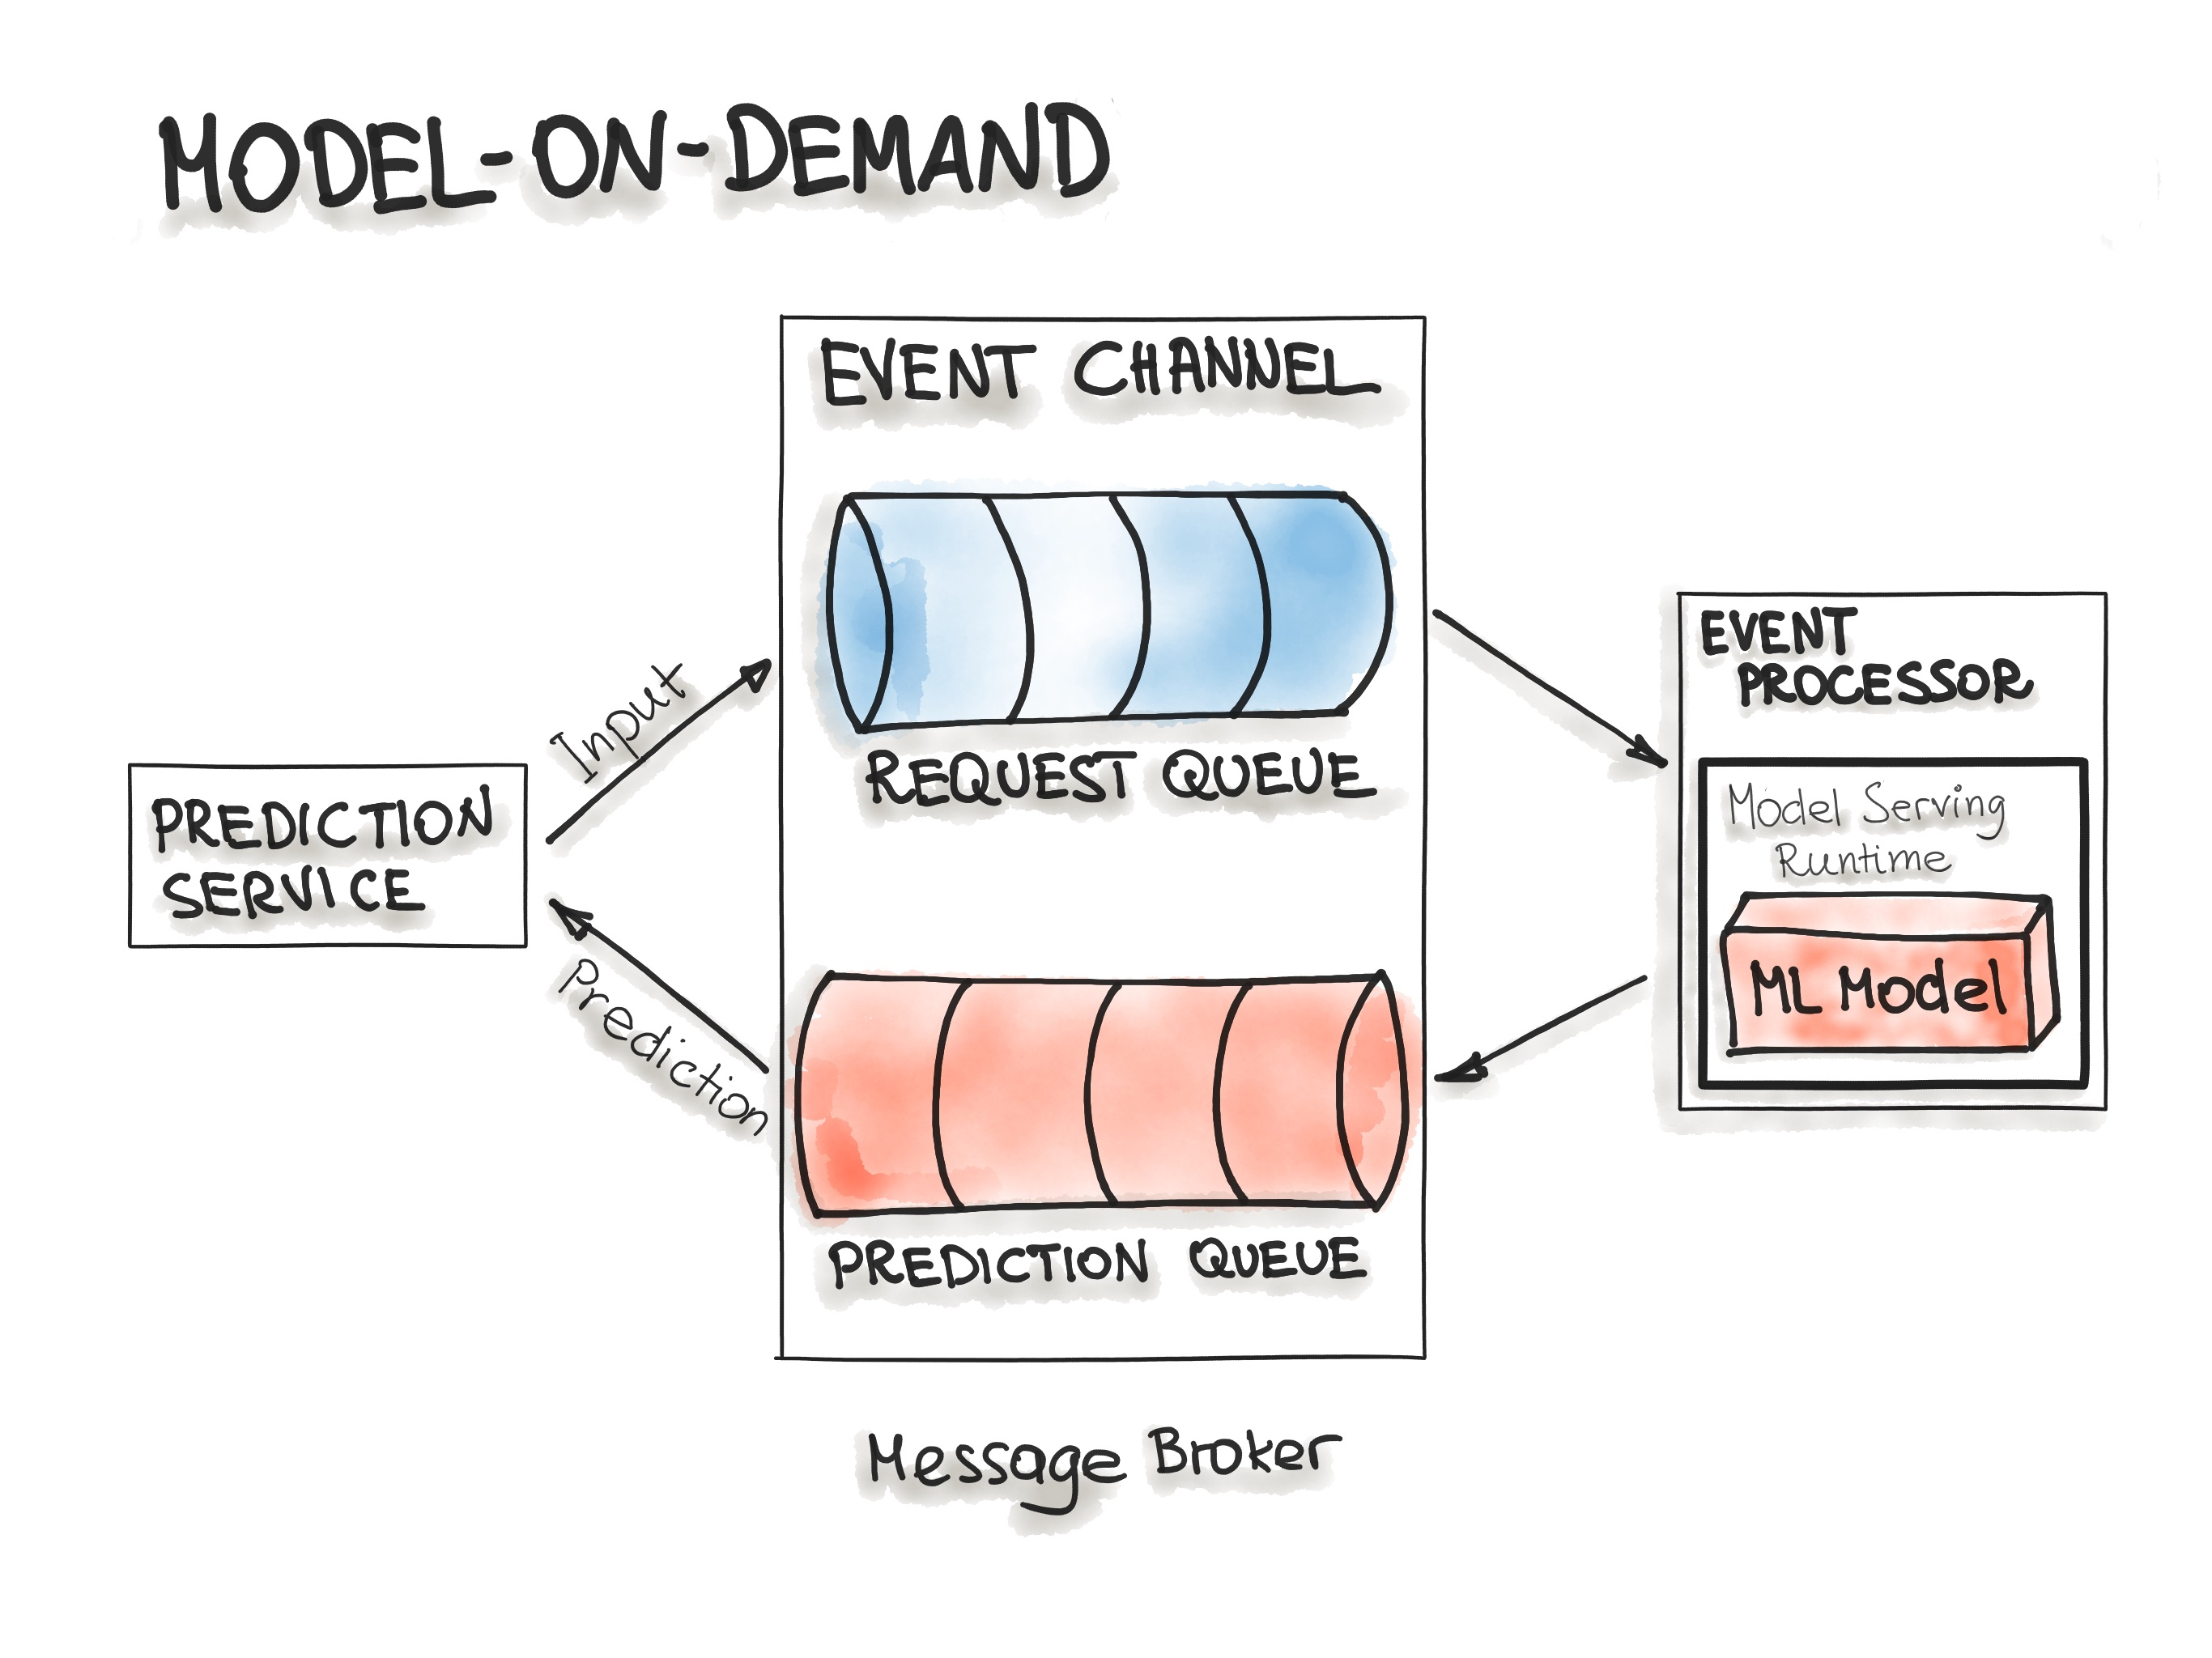
\includegraphics[width=0.8\textwidth]{02-model-on-demand.jpg}
  \caption{Ilustrasi Model-on-Demand (Sumber:~\cite{book-handsonml})}
\end{figure}

Pada dasarnya, pattern ini memiliki karakteristik yang serupa dengan Model-as-Service.
Perbedaan utamanya adalah dalam Model-as-Service, request dijalankan secara sinkron.
Dalam Model-on-Demand, terdapat penggunaan broker sehingga request terhadap model bisa dibuat asinkron.
Waktu prediksi juga bisa diatur lewat broker atau model yang digunakan.

\subsection{Hybrid Serving}

\begin{figure}
  \centering
  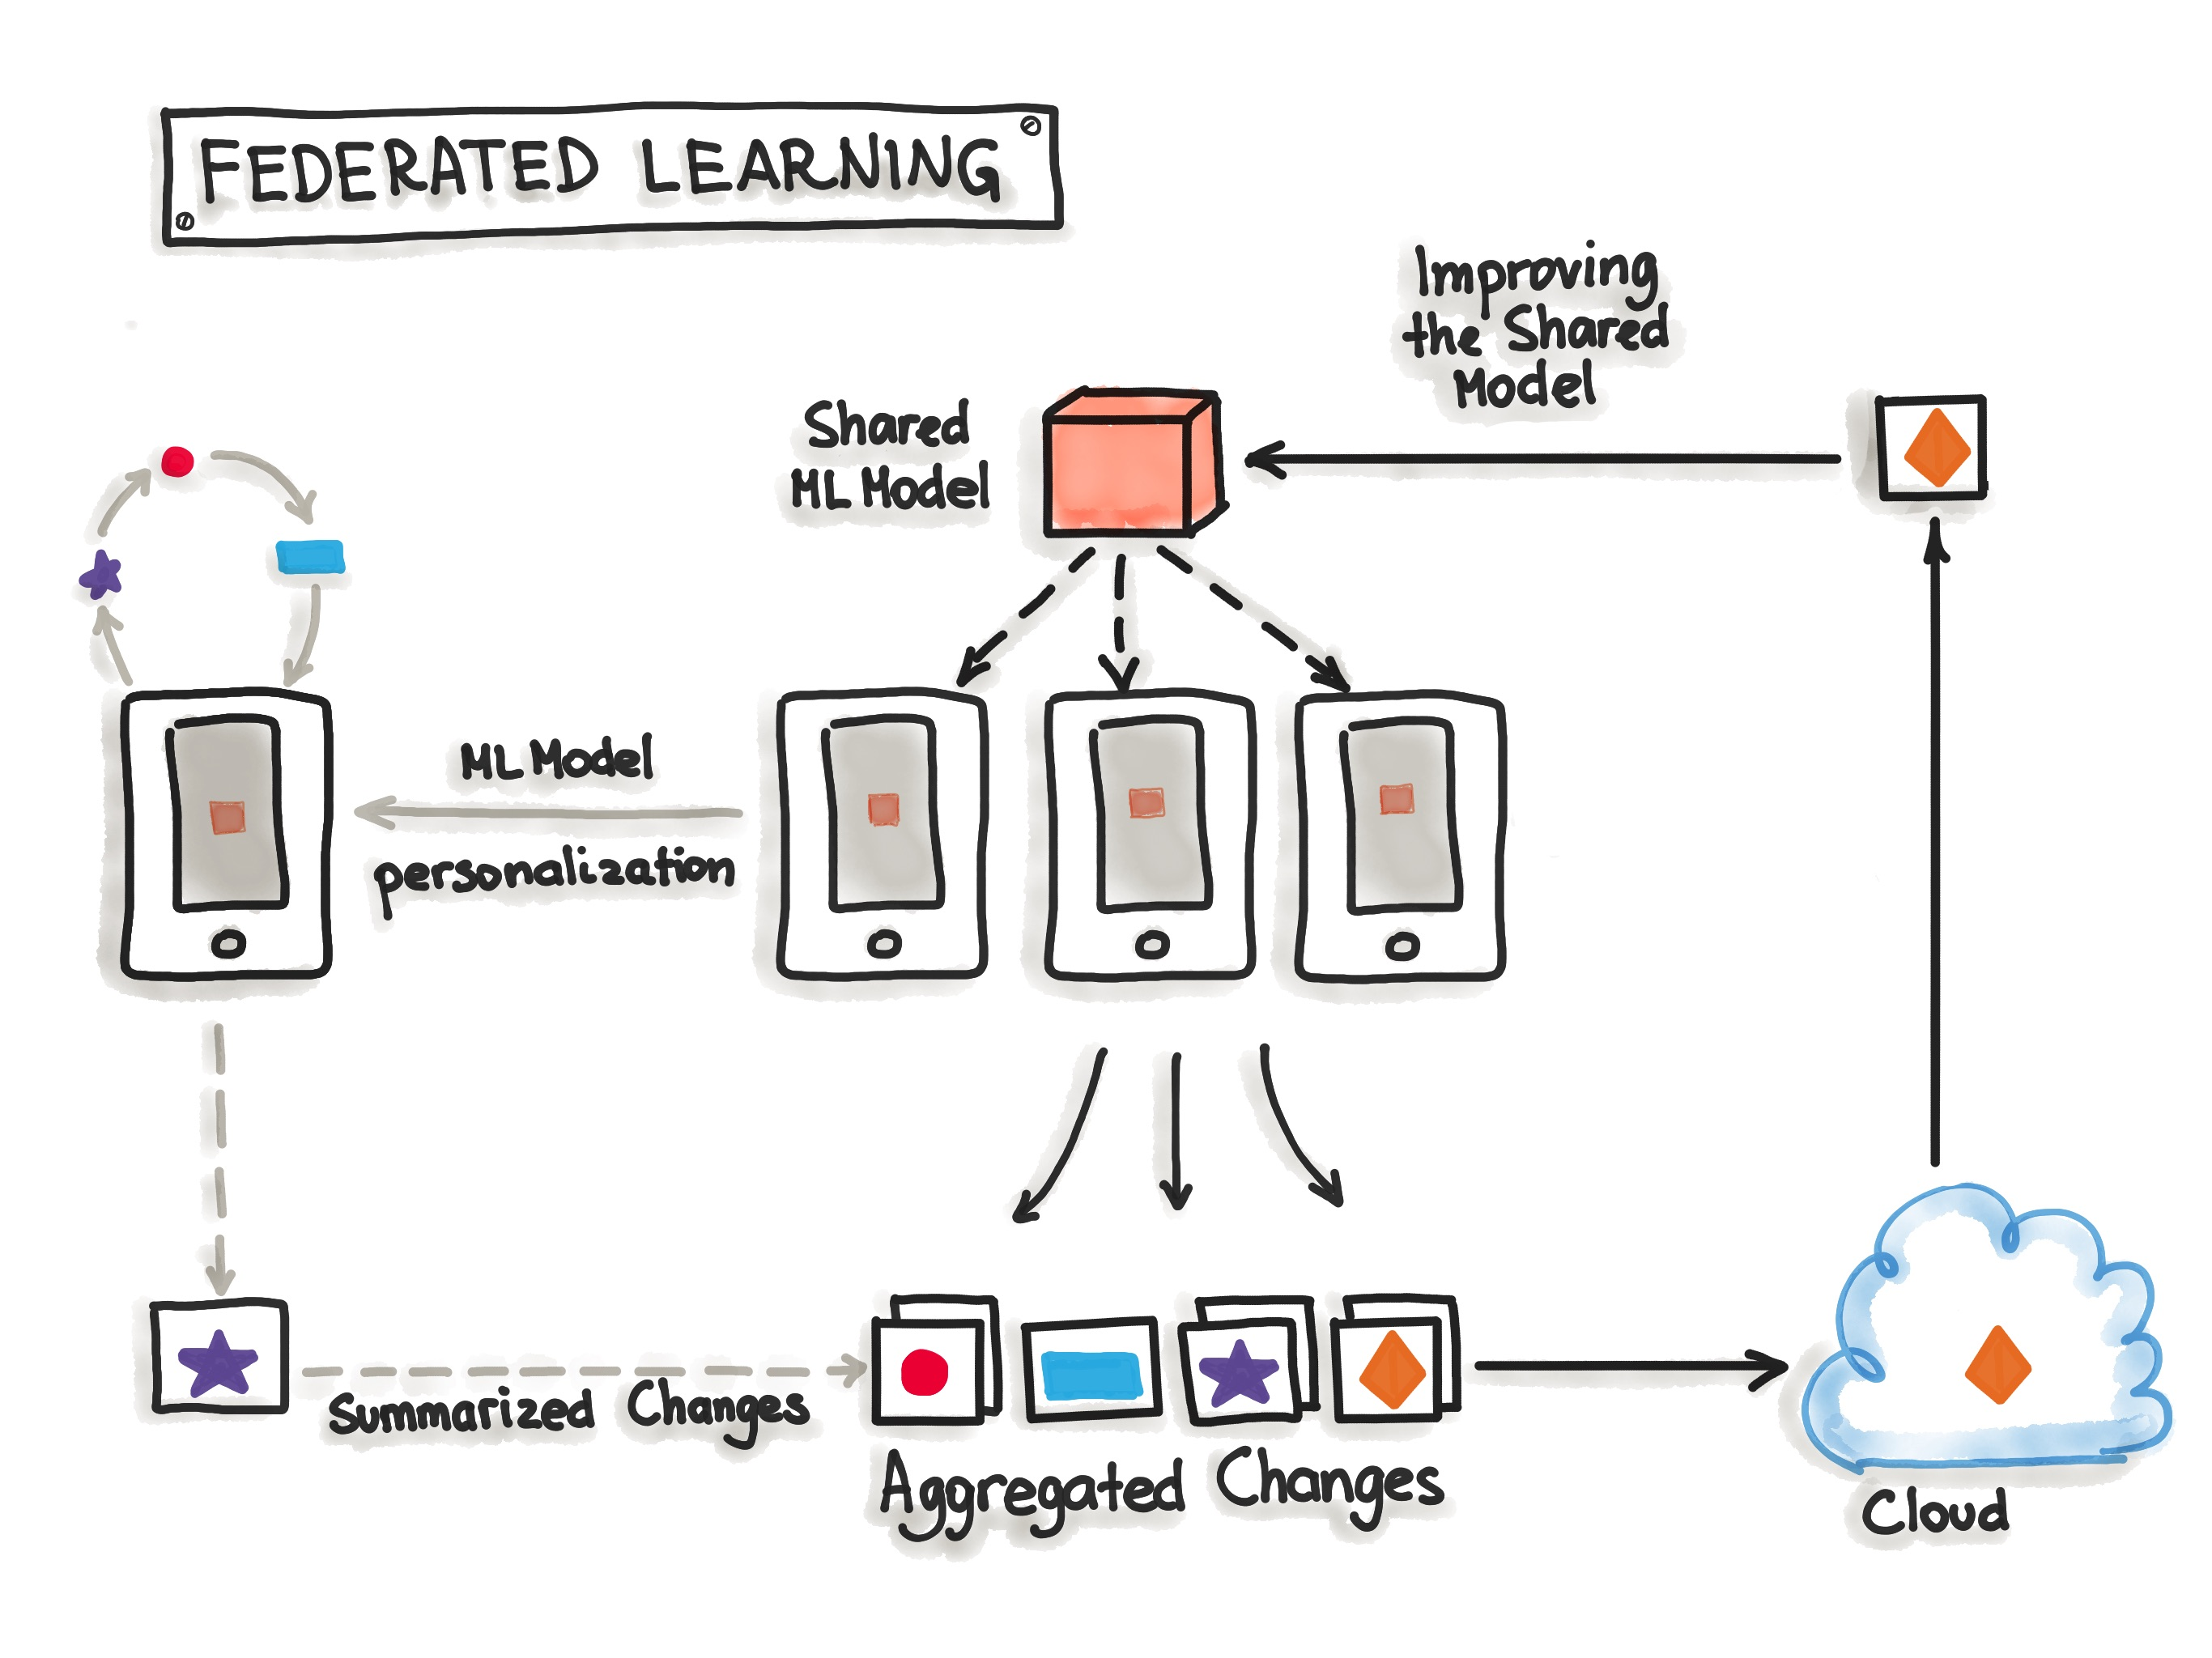
\includegraphics[width=0.8\textwidth]{02-federated-learning.jpg}
  \caption{Ilustrasi Federated Learning (Sumber:~\cite{book-handsonml})}
\end{figure}

Hybrid Serving, atau biasa dikenal dengan istilah Federated Learning adalah teknik yang memanfaatkan beberapa perangkat untuk proses trainingnya.
Model yang sudah jadi akan didistribusikan pada perangkat-perangkat berbeda, dan dari sana data baru akan dikumpulkan.
Data yang dikumpulkan akan dikirim ke sebuah central store untuk membuat model yang lebih mutakhir.

